\chapter{Experimentos y validación}
\label{chap:experimentos}

El objetivo de este capítulo es mostrar el funcionamiento de la aplicación en un caso de uso real en el que se tratará de extraer conclusiones generales acerca del consumo eléctrico de cada modelo y de si este consumo irá necesariamente acompañado de una mejora de los resultados de predicción.
Para ello se emplearán las herramientas descritas anteriormente para evaluar el consumo y el rendimiento de una serie de modelos formada por representantes de las principales familias de modelos de aprendizaje automático y recogidos en la sección~\ref{sec:models}. Estos modelos serán aplicados a los conjuntos de datos de distintas características definidos en la sección~\ref{sec:datasets}.

Durante la validación de la aplicación se llevarán acabo tres experimentos distintos.
El primero examinará el consumo energético en base al modelo seleccionado. En esta sección se tomarán varias medidas de consumo y rendimiento por modelo y conjunto de datos en una máquina con unos recursos de procesamiento concretos para analizar que modelos consumen más que otros y que características de los conjuntos de datos hacen incrementar este consumo.
El segundo consistirá en aislar un par de conjuntos de datos y tomar medidas de consumo con distintos recursos de procesado dedicados a la tarea de aprendizaje automático para observar el efecto de los recursos disponibles en el consumo energético de cada modelo.
Por último, se propondrán métodos de optimización de los modelos analizados y se examinará el efecto que pueda tener sobre su consumo. 

A través de este análisis, se pretende obtener una comprensión profunda de cómo diferentes modelos de aprendizaje automático consumen energía bajo diversas condiciones de trabajo. Este experimento también busca identificar patrones de consumo y eficiencia que puedan informar el diseño y la implementación de modelos más sostenibles y eficientes en el futuro.

\todo[inline]{Añadir esquema ???}
% What's the purpose of experiments?
% What are the expected results? More energy, more precision
% Outline / procedure / steps to follow

% 4.1 Análisis del consumo energético en base al modelo escogido
    % 4.1.1 Comparación en conjuntos de pequeño tamaño (100s - 1000s)
        % Tres conjuntos: iris, ionosphere, hepatitis
    % 4.1.2 Comparación en conjuntos de mediano tamaño (10000s)
        % Dos conjuntos: eeg-eye-state, electricity, letter, mnist_784
% 4.2 Análisis del consumo energético en base a los recursos disponibles
    % 4.2.1 Evolución del consumo con la carga del procesador
        % 1 dataset pequeño, 1 mediano
    % 4.2.2 Evolución del consumo con el aumento de recursos
        % 1 dataset grande (100000s) ?covertype?, 2-3 resource configs
% 4.3 Optimización

\section{Consumo energético basado en el modelo seleccionado}
 % - El consumo aumenta al aumentar el número de muestras
 %    1. Gráfico introductorio: número de muestras (x) vs emisiones (y), muchos modelos
 %        el consumo aumenta de forma exponencial con el número de muestras, unos modelos aumentan más que otros
 %    2. Introduce f-score: plot same lines with average f1-score instead of emissions. Los resultados son distintos, mayor consumo no implica mejor predicción
 %    3. Introduce scatter plot 4-way
    
 % - Algunos modelos son mejores que otros
 %    - Aumento de score implica aumento de consumo?
 %    - Compara average f1-score con consumo por modelo y dataset
 %    3. Introduce f-score con scatter plot 4-way, all models, 3 datasets (no average)
 %    4. Bar plot de dos datasets pequeños comparando score 

\subsubsection{Objetivos}

En esta sección se examinará el consumo energético una serie de modelos representativos aplicados a varios conjuntos de datos. El objetivo de este análisis será abordar las siguientes cuestiones clave:

\begin{itemize}
    \item Identificación de los modelos con mayor consumo energético.
    \item Determinación de los modelos cuyo consumo energético incrementa significativamente al aumentar el número de muestras.
    \item Evaluación de modelos que ofrecen mejores predicciones con menor consumo energético.
\end{itemize}

Dónde sea posible, se tratará de analizar estas cuestiones de forma general y obtener conclusiones que sean extrapolables más allá de los conjuntos de datos concretos que se hayan medido. Sin embargo, debido a la gran cantidad de variables involucradas en las variaciones de consumo entre unos casos y otros, es posible en otros conjuntos de datos se observen comportamientos distintos del consumo.

\subsubsection{Metodología}

Para analizar estas cuestiones todas las medidas de consumo serán tomadas con la aplicación desarrollada ejecutando en una misma máquina. Para cada modelo y conjunto de datos, se tomarán medidas de consumo y rendimiento utilizando validación cruzada con cinco iteraciones con un tamaño definido para los datos de testeo del 20\% del conjunto de datos. Esta técnica proporcionará una evaluación robusta y precisa tanto del comportamiento energético de los modelos como de su precisión y exactitud, ya que evitará en gran medida la presencia de valores atípicos y el riesgo de sobreajuste de los modelos.

\begin{table}[h]
    \centering
    \begin{tabular}{rl}
         Modelo & Dell XPS 15 9500\\
         Sistema Operativo & Ubuntu 20.04.6 LTS x86\_64\\
         Python & 3.12.2\\
         Procesador & Intel(R) Core(TM) i9-10885H CPU @ 2.40GHz\\
         Memoria & 7,63 GB\\
    \end{tabular}
    \caption{Características técnicas de la máquina utilizada para tomar las medidas}
    \label{tab:caracteristicas-tecnicas}
\end{table}

La aplicación será ejecutada con el siguiente comando para cada conjunto de datos distinto, en el cual \texttt{[dataset]} será sustituido por el archivo que contenga cada conjunto de datos. Adicionalmente, cualquiera de las opciones de lectura de datos descritas en la sección~\ref{sec:limpieza} podrá ser utilizada si el formato en el que se encuentren los datos lo requiere. Las características de la máquina utilizada están recogidas en la tabla~\ref{tab:caracteristicas-tecnicas}.
\begin{minted}{bash}
mlcost measure --log -cv 5 -d [dataset] [dataset-options]
\end{minted}

\subsubsection{Resultados}

La ejecución del comando anterior producirá un archivo tipo tabla de datos en formato \texttt{.csv}. La tabla~\ref{tab:medidas-1} recoge un extracto de los resultados obtenidos en el ordenador de referencia para seis conjuntos de datos distintos. El archivo completo está disponible en el repositorio de la aplicación.

\begin{table}[H]
\centerline{
\scalebox{0.78}{
\begin{tabular}{|llllllllllll|}
\hline
Dataset     & Modelo & CPU & Accuracy & Precision & F-score & Recall & Fit  & Total (s) & Emisiones & Energía  & Muestras \\
 &  & load (\%) &  & & & &  time (s) & &  (kg) &  (kWh) &  \\ \hline
Banknote    & Linear & 2.7           & 0.98      & 0.98      & 0.98    & 0.98          & 0.007             & 0.071            & 2.13E-07  & 1.10E-06 & 1372     \\
Banknote    & Linear & 2.7           & 0.97      & 0.97      & 0.97    & 0.97          & 0.006             & 0.071            & 2.13E-07  & 1.10E-06 & 1372     \\
Banknote    & Linear & 2.7           & 0.97      & 0.97      & 0.97    & 0.97          & 0.006             & 0.071            & 2.13E-07  & 1.10E-06 & 1372     \\
Banknote    & Linear & 2.7           & 0.99      & 0.99      & 0.99    & 0.99          & 0.005             & 0.071            & 2.13E-07  & 1.10E-06 & 1372     \\
Banknote    & Linear & 2.7           & 0.99      & 0.99      & 0.99    & 0.99          & 0.005             & 0.071            & 2.13E-07  & 1.10E-06 & 1372     \\
Banknote    & Forest & 2.7           & 0.99      & 0.99      & 0.99    & 0.99          & 0.184             & 1.429            & 3.27E-06  & 1.69E-05 & 1372     \\
Banknote    & Forest & 2.7           & 1.00      & 1.00      & 1.00    & 1.00          & 0.171             & 1.429            & 3.27E-06  & 1.69E-05 & 1372     \\
Banknote    & Forest & 2.7           & 0.99      & 0.99      & 0.99    & 0.99          & 0.154             & 1.429            & 3.27E-06  & 1.69E-05 & 1372     \\
Banknote    & Forest & 2.7           & 1.00      & 1.00      & 1.00    & 1.00          & 0.172             & 1.429            & 3.27E-06  & 1.69E-05 & 1372     \\
Banknote    & Forest & 2.7           & 1.00      & 1.00      & 1.00    & 1.00          & 0.158             & 1.429            & 3.27E-06  & 1.69E-05 & 1372     \\
\multicolumn{12}{|c|}{...} \\
Electricity & Neural & 102.4         & 0.82      & 0.83      & 0.83    & 0.83          & 132.768           & 518.905          & 1.19E-03  & 6.15E-03 & 45312 \\  \hline
\end{tabular}}}
\caption[Extracto de los resultados de entrenamiento]{Extracto de los resultados de entrenamiento\footnote{\url{https://github.com/l-gonz/tfg-gitt-mlcost/blob/main/model-comp-many.csv}}
\todo[inline]{Fix header format}}
\label{tab:medidas-1}
\end{table}

Cada fila en la tabla corresponde a las medidas tomadas durante una iteración de entrenamiento de cada modelo por validación cruzada. Al haber escogido utilizar validación cruzada de cinco iteraciones, la tabla de resultados cuenta con cinco filas por modelo y conjunto de datos. Sin embargo, algunas de las medidas, como la carga del procesador, el número de muestras del conjunto de datos, el tiempo total de entrenamiento, las emisiones del proceso y la energía consumida, son tomadas de forma global al finalizar todas las iteraciones de entrenamiento de cada modelo y conjunto.
Para cada iteración individual se recogen las medidas estadísticas de exactitud, precisión, exhaustividad y valor-F calculadas. Además, la implementación de validación cruzada de \texttt{scikit-learn} proporciona una medida del tiempo de entrenamiento empleado en cada iteración (fit time). Este valor puede ser utilizado junto con las emisiones y el tiempo totales de todas las iteraciones para calcular las emisiones de cada iteración de entrenamiento como muestra la ecuación~\ref{eq:fit-emissions}.

\begin{equation}
    E_1 = \frac{E_T}{t_T} \cdot t_1
    \label{eq:fit-emissions}
\end{equation}
\begin{conditions}
E_1   &   emisiones de la iteración \\
E_T   &   emisiones totales \\
t_T   &   tiempo total \\
t_1   &   tiempo de entrenamiento de la iteración
\end{conditions}

A partir de los resultados obtenidos se puede dibujar un diagrama de dispersión para visualizar cómo varían las emisiones. En la figura~\ref{fig:scatter-1} se ha utilizado el valor-F como medida de la calidad de las predicciones (eje Y), ya que es habitualmente más informativa en casos de distribuciones de clases no balanceadas. En el eje X, se han dibujado las emisiones con una escala logarítmica.

\begin{figure}[H]
  \centerline{
     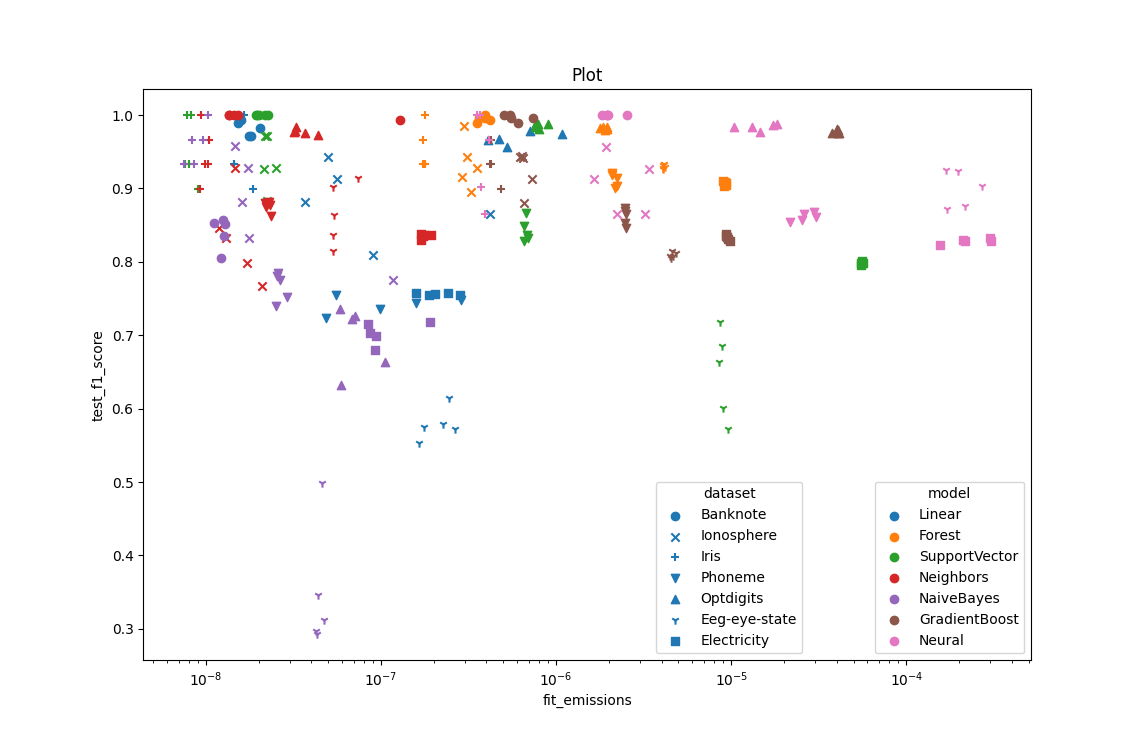
\includegraphics[width=1.3\textwidth, keepaspectratio]{img/graph/4scatter-dataset-model.png}
  }
  \caption{Valor-F alcanzado por el modelo frente a las emisiones de carbono necesarias para entrenarlo, por modelo empleado y conjunto de datos utilizado}
  \label{fig:scatter-1}
\end{figure}
\todo[inline]{Fix plot titles}

% Scatter plot bla bla bla
- Outlier eeg-eye-state lower score, high variance

- Neural, higher emissions, average score, high variance, better score more complex dataset
- Support vector, starts well, but low score for eye and very high emissions for electricity

- Forest, high score, medium emissions, even eye
- Gradient, same but a little worse on both

- Neighbors, very low emissions

- Linear, low emissions, low score
- Naive bayes, very low score, low emissions



\begin{figure}[H]
  \centerline{
     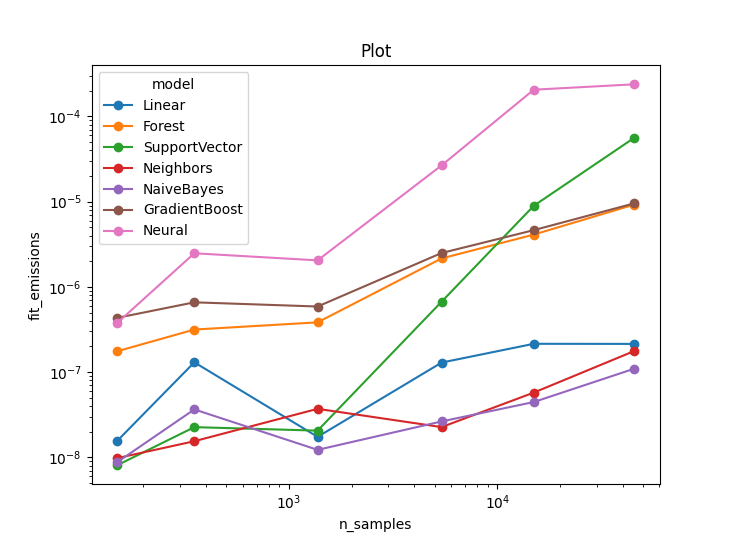
\includegraphics[width=1\textwidth, keepaspectratio]{img/graph/line-nsamples-emission-log.png}
  }
  \caption{Evolución de las emisiones de carbono con el aumento de número de muestras del conjunto de datos}
  \label{fig:line-emissions-samples}
\end{figure}
\begin{figure}[H]
  \centerline{
     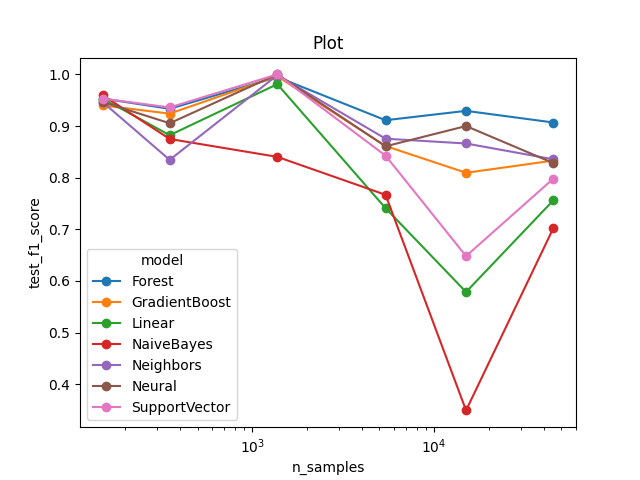
\includegraphics[width=1\textwidth, keepaspectratio]{img/graph/line-nsamples-fscore-loglin.png}
  }
  \caption{Evolución de las emisiones de carbono con el aumento de número de muestras del conjunto de datos}
  \label{fig:line-fscore-samples}
\end{figure}

- Best scores Forest, Neural, Neighbors
- Their emission: medium, high, low, in that order


\section{Consumo energético basado en los recursos disponibles}

% Datasets: 
%  - [electricity (45k) / mnist_784 (70k)] (only if poker too much),
%  - creditcard (285k), 
%  - covertype (581k), 
%  - poker-hand 1567 (1.03M)
% Models:
%  - Forest, Neural, Neighbors

% Ejecutar: (1 run instead of CV??)
 % - 1. Portatil
 % - 2. Azure (2 - 3 configs)
 % Metodología:
 % - Deploy in azure (how-to)
 % - Templates / config info
 % - Cost analysis?
 % Discusión:
 % - Compare to emission data from Azure?
 % - Bar graph/scatter plot per model/dataset

\clearpage